\subsection{Globally held chemical pairs and whole-state development}
A separately registered metadata-balanced partition closes an exposed-development coverage gap without reopening the historical evaluator. Seven canonical chemical pairs, defined by unordered names across all doses, are greedily balanced into two global panels and crossed with six whole cell lines. Twelve outer folds query each of the 54 fitting conditions once; guard rows are unused. Source sizes range from 19 to 26. Inner selection also holds a whole state and global chemical pair, retains only preregistered metadata-feasible folds, and uses no outcome-driven redraw. Exact-dose measured query singles and the legacy query-control gene-panel adaptation are explicitly permitted \citep{opaljoint2026}.
\begin{center}\small\begin{tabular}{lrrr}\toprule
Correction & Total MSE & Gain & Paired reduction interval\\\midrule
selected simple & 0.175076 & 0.00\% & [0.000000, 0.000000]\\
additive & 0.192365 & -9.88\% & [-0.040297, 0.008862]\\
mean residual & 0.201447 & -15.06\% & [-0.047645, -0.011049]\\
global correction & 0.174662 & 0.24\% & [0.000000, 0.002411]\\
single sum & 0.175103 & -0.02\% & [-0.004653, 0.004813]\\
pair product & 0.176599 & -0.87\% & [-0.010852, 0.005217]\\
mixed & 0.175353 & -0.16\% & [-0.006766, 0.006065]\\
\bottomrule\end{tabular}\end{center}
The source-selected simple reference chooses mean residual, tuned global correction or summed-single kernels by inner MSE. Pair-product and mixed kernels worsen total error by 0.87\% and 0.16\%; neither passes the registered 5\% materiality gate. Both intervals span zero. The registered 2,000 crossed state/intervention-weight bootstrap draws have 1,965 nonempty draws; their intervals condition on shared reference profiles and selection, exclude biological/refitting uncertainty, and remain diagnostic. The fixed search takes 2.16 elapsed seconds on one CPU thread, with 276.4 MB completion RSS, not a measured peak.
\par\begin{figure}[ht]\centering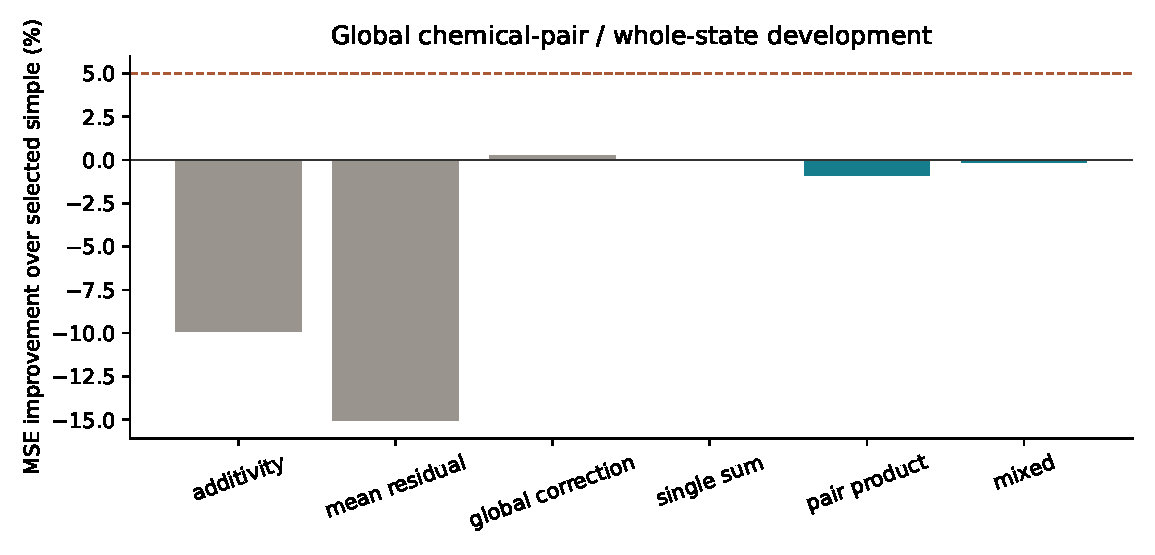
\includegraphics[width=.82\linewidth]{evidence/joint_results.pdf}\caption{Pair-specific kernels fail the joint development gate against a source-selected strong simple reference. The dashed line marks the registered 5\% screen.}\end{figure}\par
Metadata-balanced joint development is feasible here, superseding the earlier single-row lexicographic feasibility check as a development assessment. All outcomes remain exposed. This result does not supply independent joint confirmation, new independently initiated cultures, or enough sealed states to estimate biological uncertainty. No pair head, learned state encoder, risk policy, acquisition or scaling component earns advancement.
